\documentclass[12pt, conference, compsocconf]{IEEEtran}

\usepackage{amsmath, amsfonts}
\usepackage{graphicx}
\usepackage{url}
\usepackage{tikz}
\usepackage{color, soul}

%%% Package and definitions for displaying pseudocode
\usepackage{algorithm}
\usepackage[noend]{algpseudocode}
%\newcommand*\Let[2]{\State #1 $\gets$ #2}
%\algrenewcommand\alglinenumber[1]{
%    {\sf\footnotesize\addfontfeatures{Colour=888888,Numbers=Monospaced}#1}}
%\algrenewcommand\algorithmicrequire{\textbf{Precondition:}}
%\algrenewcommand\algorithmicensure{\textbf{Postcondition:}}


\begin{document}
\title{CISC-481/681 Project 3: Decision Trees}

\author{\IEEEauthorblockN{Dylan Chapp, Michael Wyatt}
\IEEEauthorblockA{Department of Computer and Information Sciences \\ University
of Delaware - Newark, DE 19716 \\ Email: \{dchapp\}, \{mwyatt\}@udel.edu}}

\maketitle

\section{Introduction}
Decision trees classifiers are a supervised machine learning technique that can achieve high accuracy, even when learning boundaries between classes that have complex geometry. 
In addition to high accuracy, decision trees can also provide fast--i.e., $O(\text{log}(n))$--query times, provided that the tree is sufficiently balanced. 

In this work we implement the ID3 algorithm for inducing decision trees from training data, using information gain of data features as our splitting heuristic. 
We test our implementation for correctness against two datasets from the UCI machine learning repository: the Auto-MPG dataset and the Wisconsin Breast Cancer dataset.
Constructing the decision tree classifiers for both of these datasets required not only correct implementation of the base algorithm, but also implementation of techniques for discretizing or ``binning" continuous-valued features.

Due to their utility and performance, optimized and well-tested implementations of machine learning algorithms such as decision trees can be found in the popular scikit-learn Python module.
In the interest of judging our implementation against a reference implementation, we perform a correctness and performance comparison of our decision tree against the scikit-learn implementation.

\section{Implementation}
We implemented a system in Python to ingest data in \texttt{.csv} form and construct a decision tree from that data using the ID3 algorithm.
Additionally, modules for discretization of non-categorical features, k-fold cross validation, and visualization of the decision tree were implemented.

\subsection{The ID3 Algorithm}
The goal of the ID3 algorithm is to construct a decision tree classifier. 
To that end, the algorithm considers subsets of the training data--initially the entire set--and selects a feature on which to partition the subset. 
Selection of a feature is equivalent to creation of a node in the tree with descendent edges for each value the feature can assume.
The algorithm then recurses on each branch; considering the subset of the training data that matches the value on the branch and excluding the previous feature from consideration.

Below in Algorithm~\ref{alg-id3}, we provide pseudocode that explicitly describes the ID3 algorithm for building a decision tree:

\begin{algorithm}
    \caption{ID3}
    \label{alg-id3}
    \begin{algorithmic}[1]
        \Function{ID3}{training data}
            \If{all training data has same class}
            \State - return a leaf node labeled with that \\ \hspace{45pt}class
            \ElsIf{there are no remaining features}
            \State - return a leaf node labeled with the \\ \hspace{45pt}majority class
            \Else
            \State - Determine the feature $f$ with \\ \hspace{45pt}maximum information gain
            \State - Generate a node labeled with that \\ \hspace{45pt}feature
            \State - Add an outgoing branch from that node \\ \hspace{45pt}for each value that feature can take
                \For{each branch}
                \State - Select subset of training data \\ \hspace{62pt}matching feature value of branch
                \State - Remove $f$ from features under \\ \hspace{62pt}consideration
                    \State - Recurse on that subset   
                \EndFor
            \EndIf
        \EndFunction
    \end{algorithmic}
\end{algorithm}

Once the tree is constructed, querying it to predict the class of a test data instance is done by traversing the tree as in binary search; choosing branches based on the values of the instance's features. 
Once a leaf node is reached, the test data instance is classified. 

\subsection{Design}
Our implementation fundamentally represents the decision tree as a set of nested Python dictionaries.
This design decision was motivated by the expected use case for a decision tree classifier--i.e., that the model will be constructed once and then queried many times.
To that end, using data structures with excellent query performance such as dictionaries is justified. 
Furthermore, the nested dictionary structure lends itself naturally to serialization--e.g., via the cPickle Python module--in the event that we want to use the model elsewhere without rebuilding it.  

\subsection{Use}
We have attempted to make building the decision tree as easy as possible.
For our implementation, the user only needs to provide the paths of the training set and the testing set as command-line arguments to the main Python script.
Optionally, the user also can specify a particular kind of discretization strategy for continuous-valued features or whether to do k-fold cross-validation. 
In any case, these features are toggled on or off via optional command-line arguments to the main Python script. 

\section{Results I: Auto-MPG Data}
The Auto-MPG dataset consists of 42 training instances, each of which has seven features: mpg, cylinders, displacement, horsepower, weight, acceleration, and model year. 
With the exception of mpg and cylinders, which are categorical, the rest of the features assume values from a continuum and therefore must be discretized prior to classification. 
We implement and test two discretization strategies and present accuracy results for each.

\subsection{Discretization of Continuous Values}
The kind of features that decision trees operate on naturally are categorical or discrete--e.g., color, shape, hasBeak--but often the data on hand, as in the case of the Auto-MPG dataset, has features that assume values from a continuum--e.g., weight or height.
For this kind of data, building a decision tree is still possible, but the data requires preprocessing via some discretization policy. 
The most obvious way to discretize is by converting the continuous feature to a simple binary feature--i.e., ``weight" $\rightarrow$ ``weight $\leq$ $t$" for some threshold $t$. 
In the interest of greater accuracy, we explore the use of two more complex discretization policies, referred to hereafter as static and dynamic.

\subsubsection{Static Discretization}
In the static policy, the discretization is done on the entire training set prior to inducing the decision tree. 
A fixed number of bins of equal width is specified and for each continuous-valued feature, the feature value is replaced by a label indicating which bin--i.e., interval--the feature value lies in. 
In this way, all continuous-valued features are converted to categorical/discrete features and the tree can be constucted as usual. 

\subsubsection{Dynamic Discretization}
One weakeness of the static policy is that since the binning is based on the full range of values that the features take on in the whole dataset, at nodes lower down in the tree the splits may not be particularly well-suited for the subsets of data associated to those nodes. 
The dynamic discretization policy remedies this by computing a binning at each node as needed, using only the data associated to that node. 
The resulting binning is in this sense better-fit to the relevant data and can yield a more accurate decision tree. 

The resulting tree is shown in Figure~\ref{fig-mpg-dt}. Observe that the maximum depth of any branch in the tree is 5 and the total number of nodes is 27--indicating that the depth $\sim$ $\text{log}_{2}($number of nodes). This balance property of the tree is expected, if not guaranteed, by the greedy splitting heuristic employed by ID3. 

\subsection{Accuracy Evaluation}
To evaluate the correctness of our decision tree, we report the recall for four cases: testing against the full training data with the static policy, testing against the full training data with the dynamic policy, testing against a separate test set with the static policy, and testing against separate test set with the dynamic policy. 
The test set was generated by taking a random sample of 10\% of the base dataset. 

Since there are three classes for the MPG dataset, the traditional definition of recall is not applicable--hence we display the results as confusion matrices. 
For all confusion matrices below, the row labels refer to the predicted class and the column labels refer to the actual class.

Table~\ref{cm-dynamic-test} contains the results from running the tree built with the dynamic discretization policy against the random sample of test data. 
Table~\ref{cm-static-test} contains the results from running the tree built with the static discretization policy against the random sample of test data. 
Table~\ref{cm-dynamic-training} contains the results from running the tree built with the dynamic discretization policy against the full set of training data. 
Table~\ref{cm-static-training} contains the results from running the tree built with the static discretization policy against the full set of training data. 

\begin{table}[h!]
\centering
\begin{tabular}{cccc}
                          & Good                   & Ok                     & Bad                    \\ \cline{2-4} 
\multicolumn{1}{c|}{Good} & \multicolumn{1}{c|}{0} & \multicolumn{1}{c|}{0} & \multicolumn{1}{c|}{1} \\ \cline{2-4} 
\multicolumn{1}{c|}{Ok}   & \multicolumn{1}{c|}{0} & \multicolumn{1}{c|}{1} & \multicolumn{1}{c|}{0} \\ \cline{2-4} 
\multicolumn{1}{c|}{Bad}  & \multicolumn{1}{c|}{0} & \multicolumn{1}{c|}{0} & \multicolumn{1}{c|}{2} \\ \cline{2-4} 
\end{tabular}
\caption{Confusion matrix for the dynamic policy vs. random sample - Accuracy = 0.75}
\label{cm-dynamic-test}
\end{table}

\begin{table}[h!]
\centering
\begin{tabular}{cccc}
                          & Good                   & Ok                     & Bad                    \\ \cline{2-4} 
\multicolumn{1}{c|}{Good} & \multicolumn{1}{c|}{0} & \multicolumn{1}{c|}{1} & \multicolumn{1}{c|}{0} \\ \cline{2-4} 
\multicolumn{1}{c|}{Ok}   & \multicolumn{1}{c|}{0} & \multicolumn{1}{c|}{0} & \multicolumn{1}{c|}{1} \\ \cline{2-4} 
\multicolumn{1}{c|}{Bad}  & \multicolumn{1}{c|}{0} & \multicolumn{1}{c|}{0} & \multicolumn{1}{c|}{2} \\ \cline{2-4} 
\end{tabular}
\caption{Confusion matrix for the static policy vs. random sample - Accuracy = 0.50}
\label{cm-static-test}
\end{table}

\begin{table}[h!]
\centering
\begin{tabular}{cccc}
                          & Good                   & Ok                      & Bad                     \\ \cline{2-4} 
\multicolumn{1}{c|}{Good} & \multicolumn{1}{c|}{8} & \multicolumn{1}{c|}{0}  & \multicolumn{1}{c|}{1}  \\ \cline{2-4} 
\multicolumn{1}{c|}{Ok}   & \multicolumn{1}{c|}{0} & \multicolumn{1}{c|}{14} & \multicolumn{1}{c|}{0}  \\ \cline{2-4} 
\multicolumn{1}{c|}{Bad}  & \multicolumn{1}{c|}{0} & \multicolumn{1}{c|}{0}  & \multicolumn{1}{c|}{15} \\ \cline{2-4} 
\end{tabular}
\caption{Confusion matrix for the dynamic policy vs. training data - Accuracy = 0.97}
\label{cm-dynamic-training}
\end{table}

\begin{table}[h!]
\centering
\begin{tabular}{cccc}
                          & Good                   & Ok                      & Bad                     \\ \cline{2-4} 
\multicolumn{1}{c|}{Good} & \multicolumn{1}{c|}{6} & \multicolumn{1}{c|}{0}  & \multicolumn{1}{c|}{1}  \\ \cline{2-4} 
\multicolumn{1}{c|}{Ok}   & \multicolumn{1}{c|}{2} & \multicolumn{1}{c|}{14} & \multicolumn{1}{c|}{3}  \\ \cline{2-4} 
\multicolumn{1}{c|}{Bad}  & \multicolumn{1}{c|}{0} & \multicolumn{1}{c|}{0}  & \multicolumn{1}{c|}{12} \\ \cline{2-4} 
\end{tabular}
\caption{Confusion matrix for the static policy vs. training data - Accuracy = 0.84}
\label{cm-static-training}
\end{table}

As demonstrated by the confusion matrices, the dynamic discretization approach greatly improves accuracy compared to the static approach. 
As expected, the decision tree does much better when tested against the exact data it was trained on, as opposed to a separate test set. 
However, in this case the disparity is exacerbated by how small both the training and test sets are. 
We expect that both recall and accuracy would improve given a larger dataset. However, it is difficult to say exactly what accuracy would be obtained before excessive overfitting occurs. 
To investigate this, we would consider taking a much larger dataset--e.g., one with more than 10,000 training instances--training on an increasing fraction of it, and monitoring the resulting accuracy. 

\begin{figure*}
  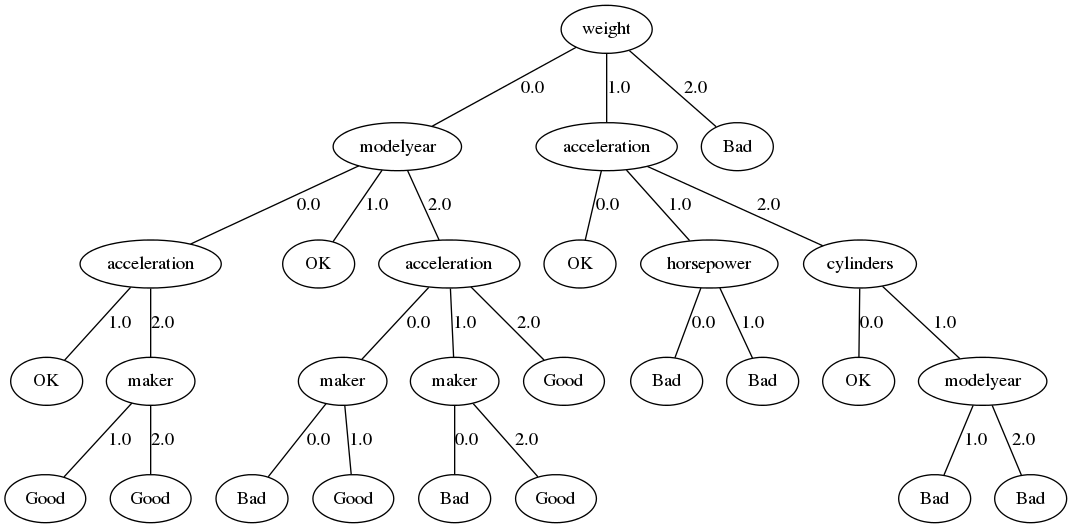
\includegraphics[width=\textwidth]{DT.png}
  \caption{The decision tree for the MPG dataset, using the static discretization policy}
  \label{fig-mpg-dt}
\end{figure*}

\section{Results II: Wisconsin Breast Cancer Data}
The Wisconsin Breast Cancer dataset is considerably larger than the Auto-MPG dataset, consisting of 419 training instances and 140 test instances, each of which has nine features. 
The features are: clump thickness, uniform cell size, uniform cell shape, marginal adhesion, single epithelial cell size, bare nuclei, bland chromatin, normal nucleoli, and mitoses--each of which assumes integer values from 1 to 10. 
Despite being essential discrete, the fact that some of these features refer to sizes and thickness indicates that their values should be discretized. Hence we employ the static and dynamic discretization policies against this dataset as well.  With the static discretization policy, we obtained a tree of depth 6 with 85 nodes.  With the dynamic discretization policy, we obtained a tree of depth 5 with 79 nodes.

\subsection{Accuracy Evaluation}
First we build the decision tree from the training data using the static discretization policy. 
Using the training data itself as the test data, we observe 86\% accuracy.
When using the test data instead, we observe 55\% accuracy.
However, when the tree is built using the dynamic discretization policy, the results are significantly improved.
Against the training data, we observe 99\% accuracy, and against the test data, we observe 93\% accuracy

\subsection{Effect of Pruning}
Pruning a decision tree classifier can be helpful when the model has suffered from overfitting--i.e., it has learned not only the underlying function that maps vectors of features to classes, but also the inherent noise in the training set. 
Due to the fact that the decision tree performed better on the training set than the testing set--i.e., 99\% accuracy vs. 93\% accuracy--we believe that the decision tree is at least somewhat overfit to the training data and would likely benefit from pruning. 

We propose pruning the decision tree in the following way. 
For each non-root and non-leaf node, replace the subtree rooted at that node by a leaf node labeled with the majority class in the subset of the training data associated with that node. 
Hence, for each such interior node, we generate a new decision tree classifier.
By testing each of those new decision trees against a \emph{validation set} set aside from both the training set and testing set, we can evaluate the fitness of each of the pruned trees. 
We would then take the pruned tree that performed best against the validation set and test it against the test set. 

\section{Extensions}

\subsection{K-fold Cross Validation}
K-fold cross validation is a technique for assessing how a model will
generalize to an independent dataset.  This technique is performed by splitting
the dataset into k partitions of roughly equal size.  A model is then built and
used to predict classes k times.  At each iteration of building and predicting,
k-1 of the partitions are used for training and the remaining partition is used
for testing.  Each of the partitions is used only once for testing.  The result
is k scores of accuracy, which can be averaged to get a better idea of model
performance with an independent dataset.

Performing 10-fold cross validation on the Wisconsin Breast Cancer training
set, we obtain the following recalls: 0.95, 0.67, 0.77, 1.0, 1.0, 0.91, 0.77,
0.86, 1.0, 0.87.  The average recall is 88\%.  This is using the same settings
as the test which gave us 99\% recall before.  However, this lower recall rate
is more accurate for how our model would perform with an independent dataset.

\subsection{Comparison with scikit-learn}
We can compare our decision tree model to the implementation in scikit-learn,
an often-used machine learning library.  Using the scikit-learn decision tree
on the Wisconsin Breast Cancer data, we can build a model using similar
parameters as we used for our model.  Additionally, we perform a 10-fold cross
validation to obtain a more realistic performance of the scikit-learn
implementation.  We obtained an average recall of 93\%.  This increase in
recall performance can be attributed to the sci-kit learn model having complex
computation to determine the best split for continuous valued features.  Our
static and dynamic methods are relatively simple in comparison.


\section{Conclusions}
We implemented a decision tree classifier that obtained highly accurate results against two data sets with diverse features.
In the process, we considered two distinct discretization policies for coping with continuous data and confirmed our hypothesis that a node-subset-level discretization policy--i.e., the dynamic policy--would outperform a global--i.e., static--discretization policy. 
We observed that decision trees can perform remarkably better in classifying the exact data they were trained on, which despite being true of essentially all machine learning algorithms, is especially relevant in the case of decision trees due to their tendency to overfit.
We also considered approaches to counteract overfitting such as pruning--which was considered theoretically--and k-fold cross validation, which was implemented. 

%\bibliographystyle{IEEEtran}
%\bibliography{bibliography}

\end{document}
